\documentclass[11pt]{article}
\usepackage[letterpaper, margin=1 in]{geometry}

\usepackage{amsmath}
\usepackage{amsfonts}
\usepackage{tikz}
\usepackage{pgfplots}
\pgfplotsset{compat=1.17}
\usepgfplotslibrary{fillbetween}

\title{Logistic Regression}
\author{}
\date{}
\setlength{\parindent}{0pt}
\begin{document}
\maketitle
\vspace{-1.2em}
With logistic regression, one of the things we might want
is for the hypothesis $h_\theta(x) \in [0, 1]$.

We'll say that our hypothesis function is equal to
some function of $g$ w.r.t $\theta^{T}x$ which can be defined as
$$\frac{1}{1 + e^{-\theta^{T}x}}$$
This is actually just a form
of the function $g(z)$, where $$g(z) = \frac{1}{1 + e^{-z}}$$

The graph of this function is a "sigmoid" or a "logistic" curve.
This forces the output values to only exist between 0 and 1.
\begin{center}
    \begin{tikzpicture}
      \begin{axis}[
        title={Logistic Curve},
        xlabel=$z$,
        ylabel=$g(z)$,
        xticklabels={,,},
      ]
        \addplot[
          color = black,
          samples = 100,
        ]{1/(1 + e^(-x))};
      \end{axis}
    \end{tikzpicture}
\end{center}
If we say that $h_\theta(x) = \theta^T x$ and force it to follow a logistic curve to constrain the output to the range $[0, 1]$, then $$P(y=1 \mid x;\theta) = h_\theta(x)$$ $$P(y=0 \mid x;\theta) = 1 - h_\theta(x)$$ where $y = \{0, 1\}$. This can be rewritten to combine these two equations as $$P(y \mid x;\theta) = h(x)^y (1 - h(x))^{1-y}$$ which uses the fact that $n^0 = 1$ and $n^1 = n$ to force the output to be $1 - h(x)$ when $y = 0$ and $h(x)$ when $y = 1$.
We can then define the likelihood of the parameters $\mathcal{L}(\theta)$ as
$$\prod_{i=1}^{m} h_\theta \left(x^{(i)}\right)^{y^{(i)}}\left(1-h_\theta \left(x^{(i)}\right)\right)^{1-y^{(i)}}$$
We then define the log likelihood to be $\ell(\theta) = \log{\mathcal{L}(\theta)}$ which is equivalent to
$$\sum_{i=1}^{m}\left[y^{(i)}\log{\left(h_\theta\left(x^{(i)}\right)\right)} + \left(1-y^{(i)}\right)\log{\left(1-h_\theta\left(x^{(i)}\right)\right)}\right]$$
We want to choose $\theta$ to maximize $\ell(\theta)$ following the maximum likelihood estimation. For this, we can use the batch gradient ascent algorithm
$$\theta_j = \theta_j + \alpha \frac{\partial}{\partial\theta}\ell(\theta)$$ which is similar to the batch gradient descent we used in the first lesson. The difference here is that we are trying to maximize $\ell(\theta)$ instead of minimize $J(\theta)$, which is why we are now adding to the parameters instead of subtracting. Instead of trying to reach a local minimum, we want to find the local maximum. Plugging in our features, target, and hypothesis function, the algorithm becomes
$$\theta_j = \theta_j + \alpha \sum_{i=1}^{m} \left(y^{(i)}-h_\theta\left(x^{(i)}\right)\right)x_j^{(i)}$$
However, gradient ascent takes quite a few iterations to converge. \hfill \\
\vspace{0em} \\
Say we have some function $f$ and want to find a $\theta$ such that $f(\theta) = 0$. What this means is that we want to maximize $\ell(\theta)$ so that ${\ell}'(\theta) = 0$. Below is a sample function $f$ we will use to demonstrate Newton's method.
\begin{center}
    \begin{tikzpicture}
      \begin{axis}[
        title={Sample Function},
        xlabel=$\theta$,
        ylabel=$f(\theta)$,
      ]
        \addplot[
          color = black,
          samples = 100,
        ]{x + exp(-2 * sin(deg(x))) + 4};
        \addplot[
          color = blue,
          only marks,
        ]coordinates{
          (4, 12.543)
        };
      \end{axis}
    \end{tikzpicture}
\end{center}
Let's say $(4, 12.543)$ is a point on this curve. This will be our first point representing $\theta^{(0)}$. This is the blue point you see in the graph.
\clearpage
The next thing we want to do is find a line tangent to to $f$ at this point; in other words, the derivative of $f$ at $\theta^{(0)}$.
\begin{center}
    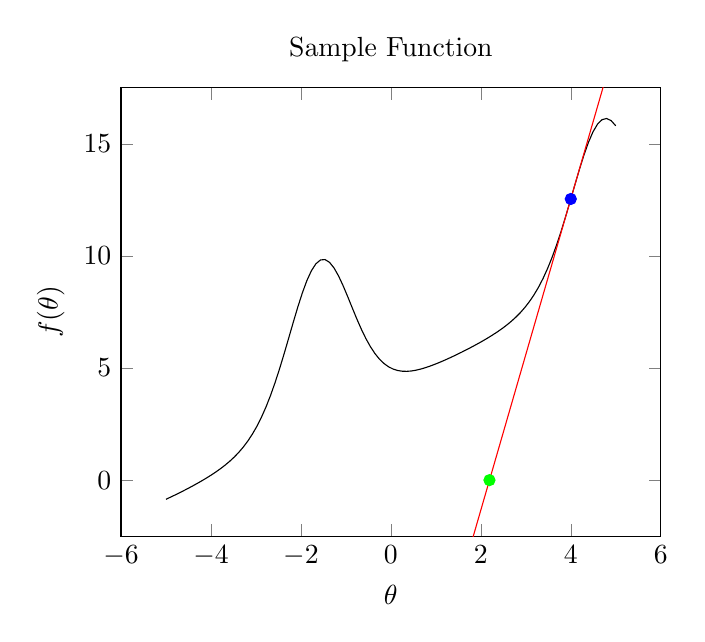
\begin{tikzpicture}
      \begin{axis}[
        title={Sample Function},
        xlabel=$\theta$,
        ylabel=$f(\theta)$,
        ymin=-2.5, ymax=17.5,
      ]
        \addplot[
          color = black,
          samples = 100,
        ]{x + exp(-2 * sin(deg(x))) + 4};
        \addplot[
          color = blue,
          only marks,
        ]coordinates{
          (4, 12.543)
        };
        \addplot[
          color = red,
          samples = 100,
        ]{6.939*(x-4)+12.543};
        \addplot[
          color = green,
          only marks,
        ]coordinates{
          (2.192, 0)
        };
      \end{axis}
    \end{tikzpicture}
\end{center}
Newton's method then sets $\theta^{(1)}$ to where our tangent line $t(\theta) = 0$, which is the green point in the above graph $(2.192, 0)$. We repeat our finding of the tangent line and look for where it crosses that horizontal axis.
\begin{center}
    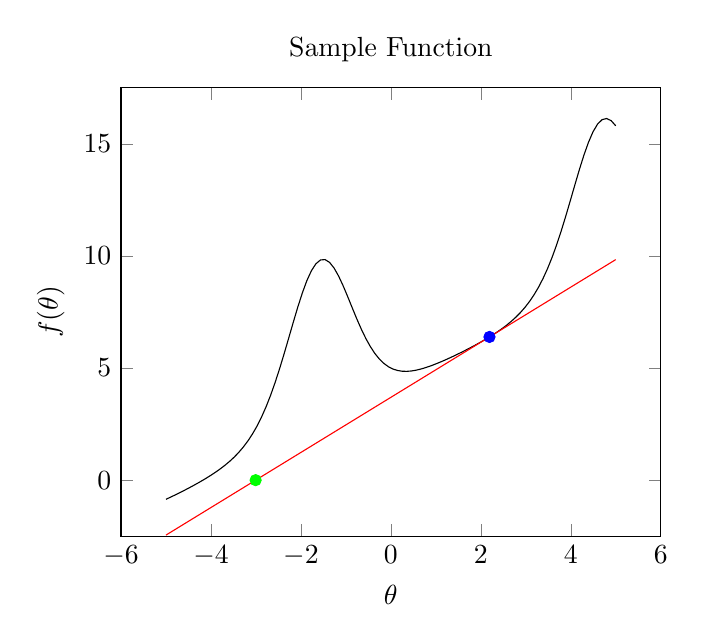
\begin{tikzpicture}
      \begin{axis}[
        title={Sample Function},
        xlabel=$\theta$,
        ylabel=$f(\theta)$,
        ymin=-2.5, ymax=17.5,
      ]
        \addplot[
          color = black,
          samples = 100,
        ]{x + exp(-2 * sin(deg(x))) + 4};
        \addplot[
          color = blue,
          only marks,
        ]coordinates{
          (2.192, 6.389)
        };
        \addplot[
          color = red,
          samples = 100,
        ]{1.229*(x-2.192)+6.389};
        \addplot[
          color = green,
          only marks,
        ]coordinates{
          (-3.007, 0)
        };
      \end{axis}
    \end{tikzpicture}
\end{center}
This continues until we reach a $\theta^{(i)}$ for which $f(\theta) = 0$.
\begin{center}
    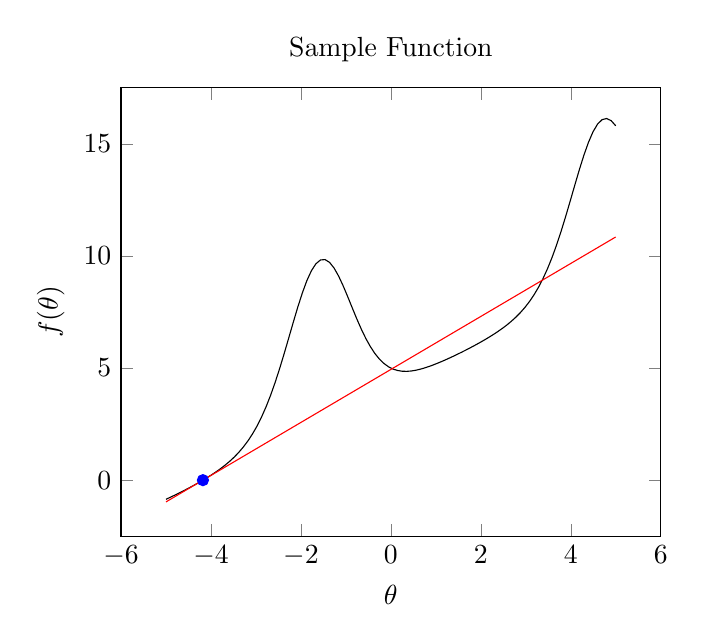
\begin{tikzpicture}
      \begin{axis}[
        title={Sample Function},
        xlabel=$\theta$,
        ylabel=$f(\theta)$,
        ymin=-2.5, ymax=17.5,
      ]
        \addplot[
          color = black,
          samples = 100,
        ]{x + exp(-2 * sin(deg(x))) + 4};
        \addplot[
          color = blue,
          only marks,
        ]coordinates{
          (-4.179, 0)
        };
        \addplot[
          color = red,
          samples = 100,
        ]{1.182*(x+4.179)};
      \end{axis}
    \end{tikzpicture}
\end{center}
As we can see, this causes our $\theta$ to converge to -4.179. Numerically, we know that $\theta^{(i+1)} = \theta^{(i)} - \Delta$ where $\Delta$ is the horizontal distance between iterations of $\theta$. We know that the slope of tangent line is ${f}'\left(\theta^{(i)}\right)$, the change in $\theta$ is $\Delta$, and the change in $f$ is $f\left(\theta^{(i)}\right)$. This relationship can be modeled as the slope formula
$${f}'\left(\theta^{(i)}\right) = \frac{f\left(\theta^{(i)}\right)}{\Delta}$$
and then rearranged to solve for $\Delta$
$$\Delta = \frac{f\left(\theta^{(i)}\right)}{{f}'\left(\theta^{(i)}\right)}$$ which allows us to conclude that the algorithm for Newton's method is
$$\theta^{(i+1)} = \theta^{(i)} - \frac{f\left(\theta^{(i)}\right)}{{f}'\left(\theta^{(i)}\right)}$$ where $f(\theta) = {\ell}'(\theta)$.
\end{document}